% задание и сама лабораторная работа
% Для листинга кода:

\lstset{ %
	language=c,                 % выбор языка для подсветки (здесь это С++)
	basicstyle=\small\sffamily, % размер и начертание шрифта для подсветки кода
	numbers=left,               % где поставить нумерацию строк (слева\справа)
	numberstyle=\tiny,           % размер шрифта для номеров строк
	stepnumber=1,                   % размер шага между двумя номерами строк
	numbersep=5pt,                % как далеко отстоят номера строк от подсвечиваемого кода
	showspaces=false,            % показывать или нет пробелы специальными отступами
	showstringspaces=false,      % показывать или нет пробелы в строках
	showtabs=false,             % показывать или нет табуляцию в строках
	frame=single,              % рисовать рамку вокруг кода
	tabsize=2,                 % размер табуляции по умолчанию равен 2 пробелам
	captionpos=t,              % позиция заголовка вверху [t] или внизу [b] 
	breaklines=true,           % автоматически переносить строки (да\нет)
	breakatwhitespace=false, % переносить строки только если есть пробел
	escapeinside={\#*}{*)}   % если нужно добавить комментарии в коде
}
\newpage
\section*{Реферат}
\addcontentsline{toc}{section}{\tocsecindent{Реферат}}

Ключевые слова: Linux, загружаемый модуль, TCP, UDP, транспортный протокол. 

Курсовой проект представляет собой загружаемый модуль ядра для управления входящими TCP/UDP пакетами (принятие или отклонение) в зависимости от выбранной политики (черный или белый список). Используется язык программирования С.

Отчёт содержит 27 страниц, 17 листингов, 8 рисунков и 7 таблиц.

\newpage
\section*{Введение}
\addcontentsline{toc}{section}{\tocsecindent{Введение}}

Транспортные протоколы предписывают способ передачи сообщений между узлами сети. Наиболее популярными из транспортных протоколов являются протокол управления передачей (TCP) и протокол пользовательских датаграмм (UDP) \cite{litlink1}. 

Входящие соединения могут использоваться злоумышленниками в корыстных целях, например, когда пользователь некорректно настроил брандмауэр в системе. 

Целью данной работы является реализация программного обеспечения для управления входящими TCP/UDP пакетами в зависимости от выбранной политики.


\newpage
\section*{Аналитическая часть}
\addcontentsline{toc}{section}{\tocsecindent{Аналитическая часть}}
В данном разделе будет произведена формализация задачи, а также будут рассмотрены способы ее решения.
\subsection*{Формализация задачи}
\addcontentsline{toc}{subsection}{\tocsecindent{Формализация задачи}}
Целью данного курсового проекта является реализация программного обеспечения, которое бы позволило управлять входящими TCP/UDP пакетами в зависимости от выбранной нами политики.

Программное обеспечение должно отслеживать и корректно идентифицировать входящие соединения, чтобы впоследствии была возможность отклонить или принять входящий пакет.

Помимо этого, необходимо разработать клиент-приложение, которое позволяло бы менять политику в реальном времени.

Таким образом, для достижения поставленной цели необходимо решить следующие задачи:
\begin{enumerate}
	\item проанализировать способы перехвата входящих TCP/UDP пакетов;
	\item разработать алгоритмы, позволяющие управлять входящими пакетами;
	\item спроектировать и реализовать модуль ядра.
\end{enumerate}

\subsection*{netfilter}
\addcontentsline{toc}{subsection}{\tocsecindent{netfilter}}

netfilter -- межсетевой экран (брандмауэр), встроен в ядро Linux с версии 2.4.

Ключевыми понятиями netfilter являются:
\begin{enumerate}
	\item правило -- состоит из критерия, действия и счетчика;
	\item цепочка -- упорядоченная последовательность правил. Стандартные цепочки указаны в таблице 1;
	\item таблица -- совокупность базовых и пользовательских цепочек, объединенных общим функциональным назначением. Существующие таблицы указаны в таблице 2.
\end{enumerate}
\begin{table}[h!]
	\caption{Типы стандартных цепочек, встроенных в систему}
	\begin{tabular}{|p{4cm}|p{12.7cm}|}
		\hline
		Название & Назначение \\
		\hline
		PREROUTING  & Для изначальной обработки входящих пакетов \\
		\hline
		INPUT & Для входящих пакетов адресованных непосредственно локальному процессу (клиенту или серверу) \\
		\hline
		FORWARD & Для входящих пакетов,перенаправленных на выход  \\
		\hline
		OUTPUT  & Для пакетов, генерируемых локальными процессами \\
		\hline
		POSTROUTING & Для окончательной обработки исходящих пакетов \\
		\hline
	\end{tabular}
\end{table}

\begin{table}[h!]
	\caption{Таблицы для организации цепочек}
	\begin{tabular}{|p{3cm}|p{13.7cm}|}
		\hline
		Название & Назначение \\
		\hline
		raw & Просматривается до передачи пакета системе определения состояний. Содержит цепочки PREROUTING и OUTPUT. \\
		\hline
		mangle & Содержит правила модификации (обычно заголовка) IP пакетов.\\
		\hline
		nat & Просматривает только пакеты, создающие новое соединение (согласно системе определения состояний) \\
		\hline
		filter & Основная таблица, используется по умолчанию если название таблицы не указано. Содержит цепочки INPUT, FORWARD, и OUTPUT. \\
		\hline
	\end{tabular}
\end{table}

Стоит также отметить, что каждый пакет может иметь одно из четырёх возможных состояний, указанных в таблице 3.
\newpage
\begin{table}[h!]
	\caption{Возможные состояния пакета}
	\begin{tabular}{|p{4cm}|p{12.7cm}|}
		\hline
		Название & Значение \\
		\hline
		NEW & Пакет открывает новый сеанс. \\
		\hline
		ESTABLISHED & Пакет является частью уже существующего сеанса \\
		\hline
		RELATED & Пакет открывает новый сеанс, связанный с уже открытым сеансом.  \\
		\hline
		INVALID & Все прочие пакеты. \\
		\hline
	\end{tabular}
\end{table}
\newpage
В целом, диаграмма прохождения пакета таблиц и цепочек принимает следующий вид (рисунок 1):
\begin{figure}[h!]\center 
	\caption{Диаграмма прохождения таблиц и цепочек}
	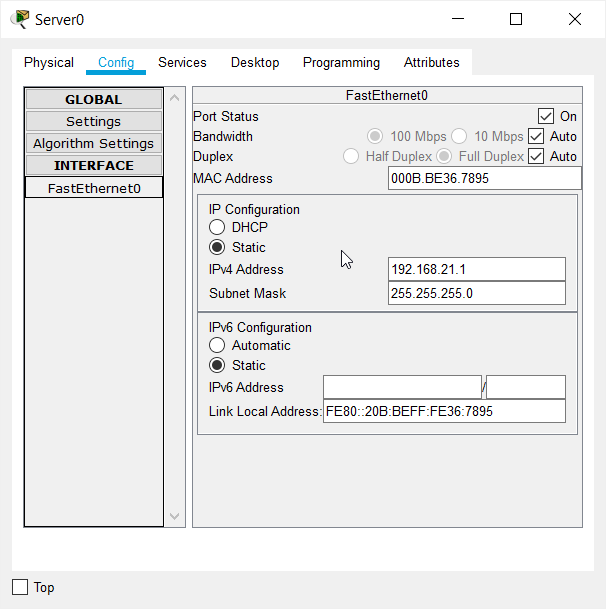
\includegraphics[scale=0.6]{1}
\end{figure}
netfilter предоставляет набор хуков (netfilter hooks) в пространстве ядра для каждого протокола (для IPv4 - 5), которые позволяют управлять пакетами соединений. Виды хуков представлены в таблице 4.

\begin{table}[h!]
	\caption{Разновидности netfilter hooks}
	\begin{tabular}{|p{6cm}|p{10.7cm}|}
	\hline
	Название & Назначение \\
	\hline
	NF\_IP\_PER\_ROUNTING & Вызывается, когда прибывает новый пакет  \\
	\hline
	NF\_IP\_LOCAL\_IN  & Вызывается в том случае, если пакет предназначен для текущей машины \\
	\hline
	NF\_IP\_FORWARD & Вызывается в случае, если пакет предназначен для другого интерфейса \\
	\hline
	NF\_IP\_POST\_ROUTING & Вызывается, когда пакет выходит за пределы машины \\
	\hline
	NF\_IP\_LOCAL\_OUT & Вызывается, когда пакет создается локально и предназначается для отправки \\
	\hline
\end{tabular}
\end{table}

Чтобы использовать хуки netfilter внутри ядра, необходимо вызывать функцию nf\_register\_hook, которая получает на вход
struct nf\_hooks\_ops.

Описание структуры nf\_hooks\_ops выглядит так:
\begin{lstlisting}[caption= struct nf\_hooks\_ops]
	struct nf_hook_ops {
		/* User fills in from here down. */
		nf_hookfn		*hook;
		struct net_device	*dev;
		void			*priv;
		u_int8_t		pf;
		unsigned int		hooknum;
		/* Hooks are ordered in ascending priority. */
		int			priority;
};
\end{lstlisting}

Поля структуры nf\_hooks\_ops описаны в таблице 5.

\begin{table}[h!]
	\caption{Структура nf\_hooks\_ops}
	\begin{tabular}{|p{5cm}|p{11.7cm}|}
	\hline
	Поле & Значение \\
	\hline
	hook & Указатель на функцию, которая вызывается при срабатывании хука. Эта функция относится к типу nf\_hookfn и возвращает NF\_DROP (отбросить пакет), NF\_ACCEPT (позволить пакету пройти дальше) или NF\_QUEUE (используется в том случае, если необходимо поставить пакет в очередь для обработки в пространстве пользователя) \\
	\hline
	hooknum & Один из идентификаторов хука (например, NF\_IP\_POST\_ROUTING). \\
	\hline
	pf & Идентификатор семейства протоколов (например, PF\_INET для IPv4). \\
	\hline
	priority & Приоритет хука (в случае, если в системе зарегистрированы другие хуки). Может принимать значение, определенное в nf\_ip\_hook\_priorities, который определен в netfilter\_ipv4.h (например, NF\_IP\_PRI\_FIRST или NF\_IP\_PRI\_RAW). \\
	\hline
\end{tabular}
\end{table}

Таким образом, netfilter hooks могут быть использованы для решения поставленной задачи.

\subsection*{Утилита iptables}
\addcontentsline{toc}{subsection}{\tocsecindent{Утилита iptables}}

iptables — утилита командной строки, является стандартным интерфейсом управления работой межсетевого экрана (брандмауэра) netfilter для ядер Linux, начиная с версии 2.4 [2]. 

Утилиту iptables можно использовать для контроля сетевых соединений. Например, для отклонения всех входящих TCP соединений, можно использовать команду: 
\begin{lstlisting}
	iptables -A INPUT -p tcp DROP
\end{lstlisting}

Однако из-за того, что для использования данной утилиты достаточно прав суперпользователя, данный способ не подходит для курсовой работы по операционным системам.

\subsection*{Загружаемый модуль ядра}
\addcontentsline{toc}{subsection}{\tocsecindent{Загружаемый модуль ядра}}

Ядро Linux динамически изменяемое -- это означает, что вы можете загружать в ядро дополнительную функциональность, выгружать функции из ядра и даже добавлять новые модули, использующие другие модули ядра. Преимущество загружаемых модулей заключается в возможности сократить расход памяти для ядра, загружая только необходимые модули (это может оказаться важным для встроенных систем).

Загружаемый модуль представляет собой специальный объектный файл в формате ELF (Executable and Linkable Format). Обычно объектные файлы обрабатываются компоновщиком, который разрешает символы и формирует исполняемый файл. Однако в связи с тем, что загружаемый модуль не может разрешить символы до загрузки в ядро, он остается ELF-объектом. Для работы с загружаемыми модулями можно использовать стандартные средства работы с объектными файлами (имеют суффикс .ko, от kernel object) [3].


В OC Linux существуют специальные команды для работы с загружаемыми модулями ядра.
\begin{enumerate}
 \item \textbf{insmod} загружает модуль в ядро из конкретного файла, если модуль зависит от других модулей. Только суперпользователь может загрузить модуль в ядро;

\item \textbf{lsmod} выводит список модулей, загруженных в ядро;

\item \textbf{modinfo} извлекает информацию из модулей ядра (лицензия, автор, описание и т.д.);

\item \textbf{rmmod} используется для выгрузки модуля из ядра, в качестве параметра передается имя файла модуля. Только суперпользователь может выгрузить модуль из ядра;

\item \textbf{dmesg} - команда для вывода буфера сообщений ядра в стандартный поток вывода. Сообщения содержат информацию о драйверах устройств, загружаемых в ядро во время загрузки системы, а также при подключении аппаратного обеспечения к системе.
\end{enumerate}
Помимо этого, загружаемые модули ядра должны содержать два макроса:\\ module\_init и module\_exit.


\subsection*{Вывод}
\addcontentsline{toc}{subsection}{\tocsecindent{Вывод}}
В данном разделе была произведена формализация задачи и рассмотрены способы ее решения. Выяснилось, что утилита iptables не подходит для решения данной задачи, поэтому мы будем использовать netfilter hooks. 
\newpage

\section*{Конструкторская часть}
\addcontentsline{toc}{section}{\tocsecindent{Конструкторская часть}}
В данном разделе будут рассмотрены требования к программе, основные сведения о реализуемых модулях, а также представлена схемы работы алгоритма.
\subsection*{Требования к программе}
\addcontentsline{toc}{subsection}{\tocsecindent{Требования к программе}}
Программное обеспечение должно состоять из загружаемого модуля ядра, который бы позволил управлять входящими TCP/UDP пакетами с помощью хуков netfilter и неподсредственно клиента, позволяющего выбирать политику управления пакетами.
\subsection*{Модуль ядра}
\addcontentsline{toc}{subsection}{\tocsecindent{Модуль ядра}}

Для начала нам необходимо инициализировать символьный драйвер, который бы позволил получать информацию с символьного устройства.

Для регистрации устройства, нужно задать специальные номера, а именно:
\begin{enumerate}
	\item MAJOR -- старший номер (является уникальным в системе);
	\item MINOR -- младший номер (не является уникальным в системе).
\end{enumerate}

Для задания cтаршего номера вызываетсяфункция register\_chrdev.
\begin{lstlisting}[caption=func register\_chrdev]
static inline int register_chrdev(unsigned int major, const char *name,
const struct file_operations *fops)
{
	return __register_chrdev(major, 0, 256, name, fops);
}
\end{lstlisting}

Также необходимо заполнить структуру file\_operations как представлено в листинге 3. Для данной работы наиболее значимой функцией является dev\_write, которая позволяет получать информацию из пространства пользователя. 
\begin{lstlisting}[caption= struct file\_operations для текущей задачи, label = 1]
static struct file_operations fops =
{
	.open = devel_open,
	.write = dev_write,
	.release = dev_release,
};
\end{lstlisting}

\begin{lstlisting}[caption= функции struct file\_operations, label = 2]
static int     devel_open(struct inode *, struct file *);
static int     dev_release(struct inode *, struct file *);
static ssize_t dev_write(struct file *, const char *, size_t, loff_t *); 
\end{lstlisting}

Для хранения информации о текущей политике выделяется двумерный массив символов, который также позволяет журналировать предыдущие изменения политики.

\begin{lstlisting}[caption=Массив для хранения изменений политики]
char list[100][6];
int listIterator = 0;
\end{lstlisting}

Как уже было упомянуто ранее, следующим шагом будет необходимо вызвать функцию nf\_register\_hook и передать в нее инициализированную структуру nf\_hooks\_ops.

Поскольку наша задача заключается в том, чтобы перехватить все входящие пакеты, поле hooknum должно принимать значение NF\_IP\_LOCAL\_IN (в нашем случае NF\_INET\_LOCAL\_IN, поскольку мы работаем только с протоколами TCP, UDP). Тогда структура nf\_hooks\_ops в нашем случае примет следующий вид:
\begin{lstlisting}[caption= struct nf\_hooks\_ops для текущей задачи]
static struct nf_hook_ops drop __read_mostly = {
.pf = NFPROTO_IPV4,
.priority= NF_IP_PRI_FIRST,
.hooknum = NF_INET_LOCAL_IN,
.hook = (nf_hookfn *) icmp_hook
};
\end{lstlisting}
\newpage
Листинг вышеупомянутой функции представлен ниже.

\begin{lstlisting}[caption= func nf\_register\_hook]
int nf_register_net_hook(struct net *net, const struct nf_hook_ops *reg)
{
int err;

if (reg->pf == NFPROTO_INET) {
...
} else {
err = __nf_register_net_hook(net, reg->pf, reg);
if (err < 0)
return err;
}

return 0;
}
\end{lstlisting}

Функция icmp\_hook, которая вызывается при срабатывании хука, будет представлена дальше (Технологическая часть, листинг 17).

Для корректного журналирования полезно будет определить IP адрес и порт приходящего пакета для того, чтобы принять или отклонить его в зависимости от установленной политики. Нам понадобятся функции skb\_transport\_header и skb\_network\_header, в которые мы передадим struct sk\_buff.

\begin{lstlisting}[caption= struct sk\_buff]
struct sk_buff {
	union {unnamed_union};
	...
	sk_buff_data_t tail;
	sk_buff_data_t end;
	unsigned char * head;
	unsigned char * data;
	...
}; \end{lstlisting}

Некоторые поля структуры sk\_buff описаны в таблице 6.
\newpage
\begin{table}[h!]
	\caption{Структура sk\_buff}
	\begin{tabular}{|p{5cm}|p{11.7cm}|}
		\hline
		Поле & Значение \\
		\hline
		head & Указывает на начало выделенного пространства \\
		\hline
		data & Указывает на начало достоверных октетов \\
		\hline
		tail & Является окончанием достоверных октетов \\
		\hline
		end & Указывает на максимальный адрес, который может достичь tail \\
		\hline
	\end{tabular}
\end{table}

Ниже представлены листинги вышеупомянутых функций.
\begin{lstlisting}[caption= func skb\_transport\_header]
static inline unsigned char *skb_transport_header(const struct sk_buff *skb)
{
	return skb->head + skb->transport_header;
}\end{lstlisting}
\begin{lstlisting}[caption= func skb\_network\_header]
static inline unsigned char *skb_network_header(const struct sk_buff *skb)
{
	return skb->head + skb->network_header;
}
\end{lstlisting}

Наконец, останется только принять или отклонить пакет c помощью необходимого флага.

В рамках данной курсовой работы достаточно использовать NF\_ACCEPT и NF\_DROP.

\begin{table}[h!]
	\caption{Флаги netfilter}
	\begin{tabular}{|p{5cm}|p{11.7cm}|}
		\hline
		Флаг & Значение \\
		\hline
		NF\_ACCEPT & Позволить пакету продолжить перемещение\\
		\hline
		NF\_DROP & Отбросить пакет \\
		\hline
		NF\_STOLEN & Перехватить перемещение \\
		\hline
		NF\_QUEUE & Поместить пакет в очередь \\
		\hline
		NF\_REPEAT & Вызвать хук снова \\
		\hline
	\end{tabular}
\end{table}


\subsection*{Клиент-приложение}
\addcontentsline{toc}{subsection}{\tocsecindent{Клиент-приложение}}

Клиент-приложение должно обращаться непосредственно к созданному нами символьному устройству.

\begin{lstlisting}
fd = open("/dev/pd", O_RDWR);
if (fd < 0)
{
	printf("failed to open the device...");
	return -1;
}
\end{lstlisting}

Запись в файл производится с помощью команд lseek и write.

\newpage
\subsection*{Схемы, демонстрирующие работу модуля}
\addcontentsline{toc}{subsection}{\tocsecindent{Схемы, демонстрирующие работу модуля}}
Ниже представлены схемы, демонстрирующие работу модуля.

\begin{figure}[h!]\center 
	\caption{Cхема инициализации работы модуля}
	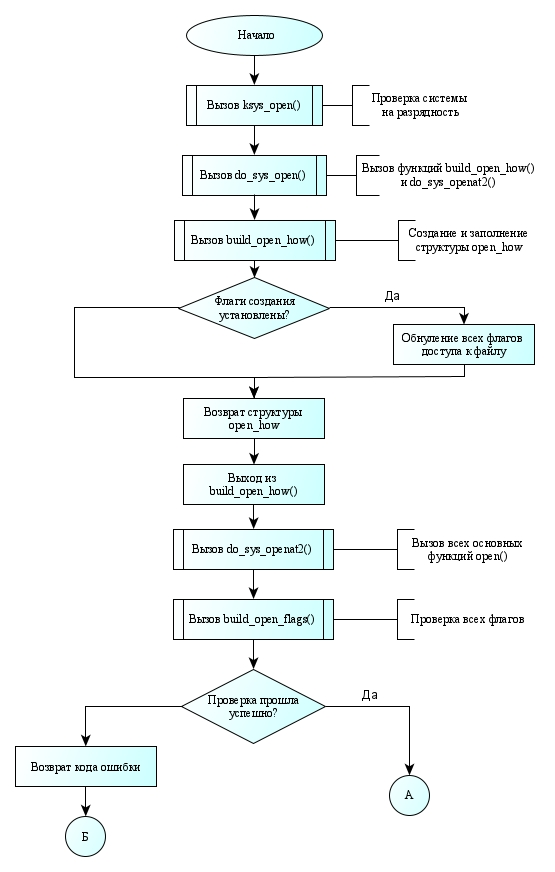
\includegraphics[scale=0.55]{1.jpg}
\end{figure}

\newpage
\begin{figure}[h!]\center 
	\caption{Cхема инициализации работы модуля}
	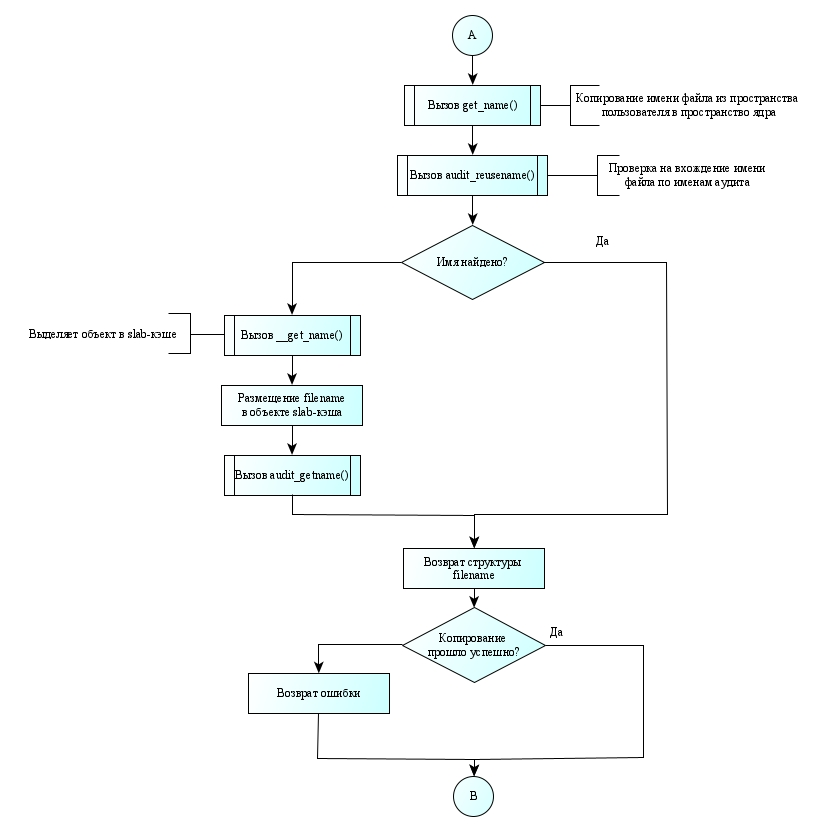
\includegraphics[scale=0.65]{2.jpg}
\end{figure}

\newpage
\begin{figure}[h!]\center 
	\caption{Cхема обработки пакетов}
	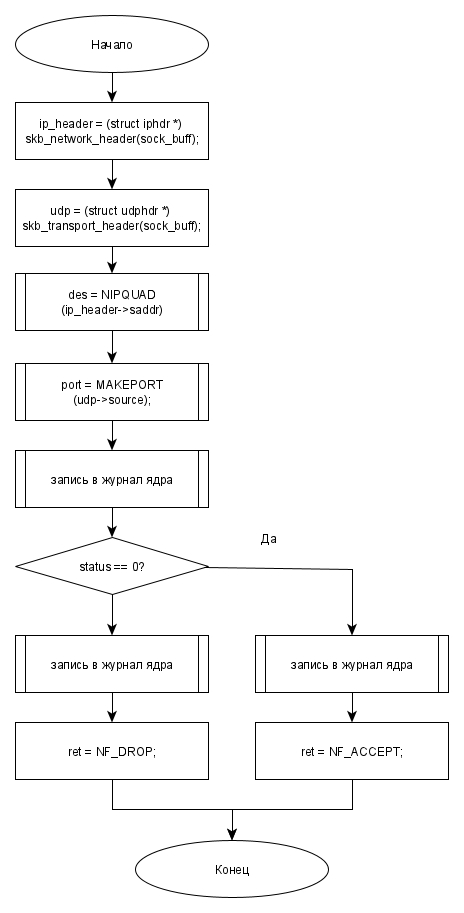
\includegraphics[scale=0.65]{3.jpg}
\end{figure}

\newpage
\begin{figure}[h!]\center 
	\caption{Cхема завершения работы модуля}
	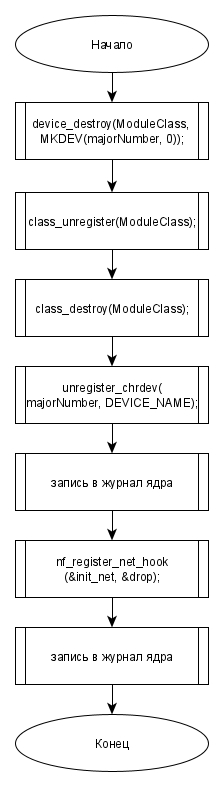
\includegraphics[scale=0.75]{4.jpg}
\end{figure}

\subsection*{Вывод}
\addcontentsline{toc}{subsection}{\tocsecindent{Вывод}}
В данном разделе были рассмотрены требования к программе, основные сведения о реализуемых модулях, предоставлены схемы, описывающие работу модуля.

\section*{Технологическая часть}
\addcontentsline{toc}{section}{\tocsecindent{Технологическая часть}}
В данном разделе будет предоставлен листинг реализованных модулей и проведена апробация.
\subsection*{Выбор языка программирования и среды разработки}
\addcontentsline{toc}{subsection}{\tocsecindent{Выбор языка программирования и среды разработки}}
В качестве языка программирования был выбран C, поскольку при помощи этого языка реализованы все модули ядра и драйверы в OC Linux.

В качестве среды разработки был выбран стандартный текстовый редактор ОС Linux.

\subsection*{Содержимое Makefile}
\addcontentsline{toc}{subsection}{\tocsecindent{Содержимое Makefile}}
Ниже представлено содержимое Makefile.
\begin{lstlisting}[caption = Содержимое Makefile]
obj-m += pd.o

all:
	make -C /lib/modules/$(shell uname -r)/build/ M=$(PWD) modules
clean:
	make -C /lib/modules/$(shell uname -r)/build/ M=$(PWD) clean\end{lstlisting}
	
\subsection*{Описание некоторых моментов реализации}
\addcontentsline{toc}{subsection}{\tocsecindent{Описание некоторых моментов реализации}}
В листинге 12 производится инициализация модуля ядра с помощью макросов входа/выхода, в листинге 13 показаны макросы модуля, а в листингах 14 и 15 продемонстрированы констуктор и деструктор модуля.

\begin{lstlisting}[caption = Инициализация модуля ядра]
module_init(pd_init);
module_exit(pd_exit);
\end{lstlisting}

\begin{lstlisting}[caption = Макросы модуля]
MODULE_LICENSE("GPL");
MODULE_AUTHOR("Furdik Nikita");
MODULE_DESCRIPTION("TCP/UDP packet manager");
MODULE_VERSION("1.0");
\end{lstlisting}
\newpage
\begin{lstlisting}[caption = Констуктор модуля]
static int __init pd_init(void) {
	printk(KERN_INFO "packet manager :: initializing the device driver\n");
	
	majorNumber = register_chrdev(0, DEVICE_NAME, &fops);
	if (majorNumber < 0){
		printk(KERN_ALERT "packet manager :: device failed to register a major number\n");
		return majorNumber;
	}
	printk(KERN_INFO "packet manager :: device registered correctly with a major number %d\n", majorNumber);
	ModuleClass = class_create(THIS_MODULE, CLASS_NAME);
	if (IS_ERR(ModuleClass)){
		unregister_chrdev(majorNumber, DEVICE_NAME);
		printk(KERN_ALERT "packet manager :: failed to register device class\n");
		return PTR_ERR(ModuleClass);
	}
	printk(KERN_INFO "packet manager :: device class registered correctly\n");
	ModuleDevice = device_create(ModuleClass, NULL, MKDEV(majorNumber, 0), NULL, DEVICE_NAME);
	if (IS_ERR(ModuleDevice)){
		class_destroy(ModuleClass);
		unregister_chrdev(majorNumber, DEVICE_NAME);
		printk(KERN_ALERT "packet manager :: Failed to create the device\n");
		return PTR_ERR(ModuleDevice);
	}
	printk(KERN_INFO "packet manager :: device class created correctly\n");
	printk(KERN_INFO "starting the device!\n");
	nf_register_net_hook(&init_net,&drop);
	return 0;
}\end{lstlisting}
\begin{lstlisting}[caption = Деструктор модуля]
static void __exit pd_exit(void) {
device_destroy(ModuleClass, MKDEV(majorNumber, 0));
class_unregister(ModuleClass);
class_destroy(ModuleClass);
unregister_chrdev(majorNumber, DEVICE_NAME);
printk(KERN_INFO "packet manager :: stopping the device!\n");
nf_unregister_net_hook(&init_net, &drop);

}

\end{lstlisting}

Далее покажем функции структуры file\_operations.

\begin{lstlisting}[caption = Функции структуры file\_operations]
static int devel_open(struct inode *inodep, struct file *filep){
	numberOpens++;
	printk(KERN_INFO "packet manager :: device has been opened %d time(s)\n", numberOpens);
	return 0;
}


static ssize_t dev_write(struct file *filep, const char *buffer, size_t len, loff_t *offset){
	sprintf(list[listIterator], "%s", buffer);   
	printk(KERN_INFO "packet manager :: received from the user: %s mode \n", list[listIterator]);
	if(!strcmp(list[listIterator], "white")){
		mode = 1;
		listIterator = 0;
	}else if(!strcmp(list[listIterator], "black")){
		mode = 0;
		listIterator = 0;	
	}else{
		listIterator++;
	}	
	return sizeof(list[listIterator]);
}


static int dev_release(struct inode *inodep, struct file *filep){
	printk(KERN_INFO "packet manager :: device successfully closed\n");
	return 0;
}\end{lstlisting}

И, наконец, опишем функцию icmp\_hook, которая вызывается при срабатывании хука.
\begin{lstlisting}[caption=func icmp\_hook]
unsigned int icmp_hook(unsigned int hooknum, struct sk_buff *skb, 
const struct net_device *in, const struct net_device *out, int(*okfn)(struct sk_buff *)) {
	int port;
	char des[100];
	
	sock_buff = skb;
	
	ip_header = (struct iphdr *) skb_network_header(sock_buff);
	udp = (struct udphdr *) skb_transport_header(sock_buff);
	
	port = MAKEPORT(udp->source);
	
	sprintf(des, "%d.%d.%d.%d:%d",NIPQUAD(ip_header->saddr), port);
	printk(KERN_INFO "packet manager :: a packet was recieved from %s\n",des);
	printk(KERN_INFO "packet manager :: we are in %s mode\n", mode == 0 ? "black list" : "white list");

	int status = 0;
	if(mode == 1)
	status = 1;

	if(status == 1){
		printk(KERN_INFO "packet manager :: packet has been accepted!");
		return NF_ACCEPT;
	}
	else{
		printk(KERN_INFO "packet manager :: dropping the packet!");
		return NF_DROP;	
	}
}
\end{lstlisting}
\newpage
\subsection*{Пример работы загружаемого модуля}
\addcontentsline{toc}{subsection}{\tocsecindent{Пример работы загружаемого модуля}}

Загрузим модуль ядра и проверим его успешную загрузку.
\begin{figure}[h!]\center 
	\caption{Загрузка модуля}
	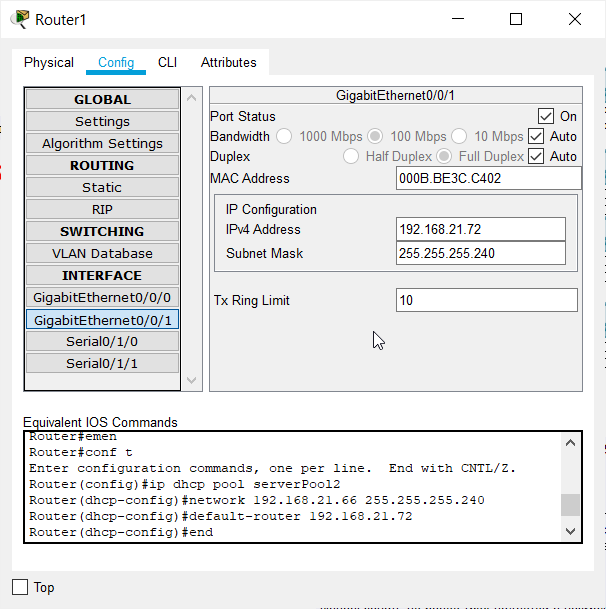
\includegraphics[scale=1]{4}
\end{figure}

Изначально устанавливается политика черного списка, т.е. все входящие пакеты отклоняются, как видно из рисунка 6.

Запустим клиент и изменим политику. В случае неудачного открытия драйвера устройства, мы увидим сообщение об ошибке (рисунок 7).

\begin{figure}[h!]\center 
\caption{Неудачный запуск клиента}
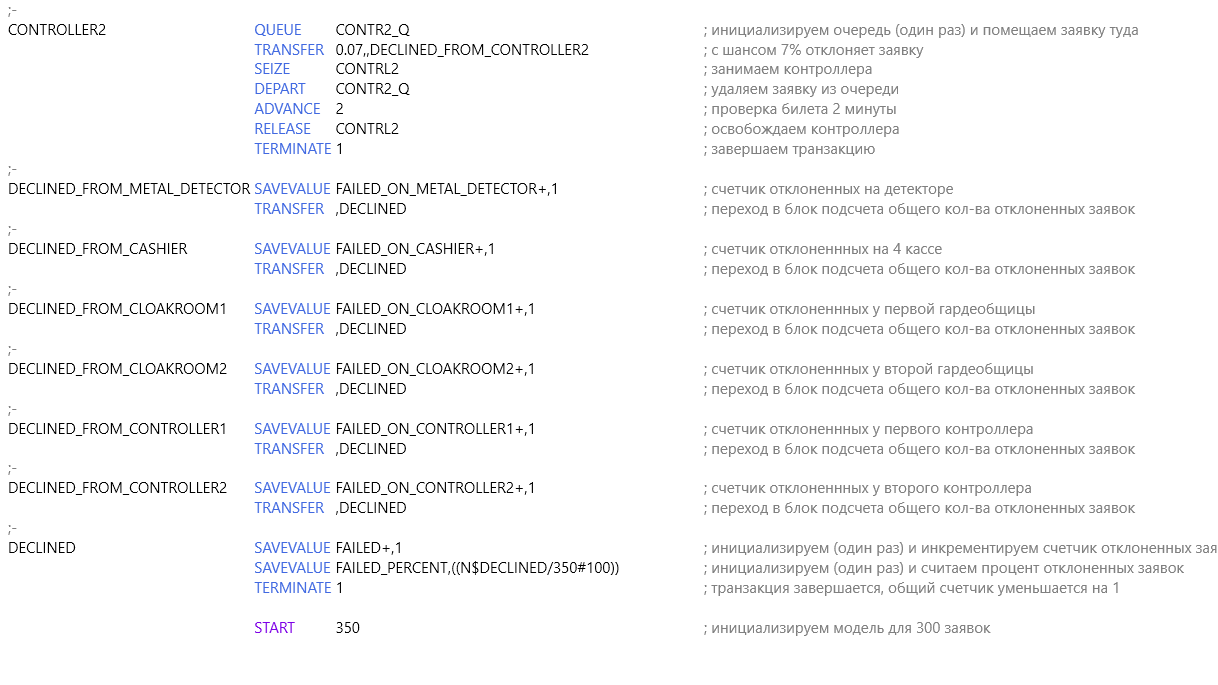
\includegraphics[scale=0.8]{5}
\end{figure}

Успешное изменение политики представлено на рисунке 8.
\newpage
\begin{figure}[h!]\center 
	\caption{Смена политики принятия пакетов}
	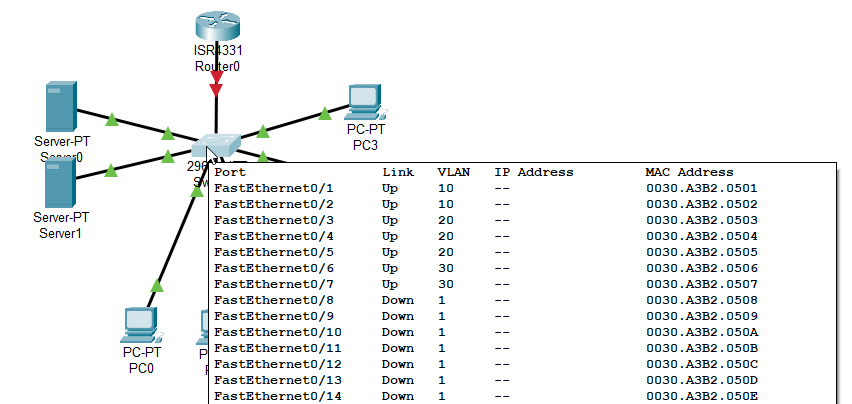
\includegraphics[scale=0.37]{6}
\end{figure}

\subsection*{Вывод}
\addcontentsline{toc}{subsection}{\tocsecindent{Вывод}}
Были реализованы модуль ядра и приложение-клиент, листинги которых были предоставлены в данном разделе. Помимо этого, программное обеспечение было протестировано на наличие ошибок.

\newpage

\section*{Заключение}
\addcontentsline{toc}{section}{\tocsecindent{Заключение}}

Во время выполнения курсового проекта были достигнуты поставленные цель и задачи: проанализированы способы перехвата входящих TCP/UDP пакетов, разработаны алгоритмы, позволяющие управлять входящими пакетами, а также  спроектирован и реализован загружаемый модуль ядра.

В ходе выполнения поставленных задач были изучены возможности языка C, получены знания в области написания загружаемых модулей ядра и драйверов.
% список литературы
\newpage
\addcontentsline{toc}{section}{\tocsecindent{Список литературы}}

\begin{thebibliography}{}
    \bibitem{litlink1}  Население Земли. [Электронный ресурс]. – Режим доступа: http://www.countrymeters.info (дата обращения 30.05.2020)
    \bibitem{litlink2}  Дефицит пресной воды в странах мира. Справка. [Электронный ресурс]. – Режим доступа:  https://ria.ru/20100322/215718166.html (дата обращения 30.05.2020)
     \bibitem{litlink3} ДЕФИЦИТ ПРЕСНОЙ ВОДЫ: ПРОБЛЕМЫ И СПОСОБЫ РЕШЕНИЯ [Электронный ресурс]. – Режим доступа: 
    https://thewallmagazine.ru/lack-of-fresh-water/ (дата обращения 30.05.2020)
  \bibitem{litlink4} Water scarcity [Электронный ресурс]. – Режим доступа:  https://en.wikipedia.org/wiki/Water\_scarcity (дата обращения 30.05.2020)
  \bibitem{litlink5}Конференция "Международное десятилетие снабжения питьевой водой и санитарии". [Электронный ресурс]. – Режим доступа:  https://documents-dds-ny.un.org/doc/RESOLUTION/GEN/NR0/394/93/IMG/NR039493.pdf?OpenElement 
  \bibitem{litlink6} Всемирный доклад ООН.[Электронный ресурс]. – Режим доступа: \\ https://unesdoc.unesco.org/ark:/48223/pf0000231823\_eng
\end{thebibliography}

\newpage
\section*{Приложение А}
\addcontentsline{toc}{section}{\tocsecindent{Приложение А}}

\begin{lstlisting}
#include <linux/kernel.h>
#include <linux/module.h>
#include <linux/netfilter.h>
#include <linux/netfilter_ipv4.h>
#include <linux/skbuff.h>
#include <linux/udp.h>
#include <linux/icmp.h>
#include <linux/ip.h>
#include <linux/inet.h>
#include <linux/init.h>
#include <linux/device.h>
#include <linux/fs.h>
#include <linux/uaccess.h>


#define  DEVICE_NAME "pd"
#define  CLASS_NAME  "pd"
#define NIPQUAD(addr) ((unsigned char *)&addr)[0], ((unsigned char *)&addr)[1], ((unsigned char *)&addr)[2], ((unsigned char *)&addr)[3]
#define MAKEPORT(port) ((unsigned char *)&port)[0] * 256 + ((unsigned char *)&port)[1]

MODULE_LICENSE("GPL");
MODULE_AUTHOR("Furdik Nikita");
MODULE_DESCRIPTION("TCP/UDP packet manager");
MODULE_VERSION("1.0");


char list[100][100];
int listIterator = 0;
int mode = 0; //0 == black and 1 == white

static int    majorNumber;
static int    numberOpens = 0;
static struct class *  ModuleClass  = NULL;
static struct device * ModuleDevice = NULL;

static int     devel_open(struct inode *, struct file *);
static int     dev_release(struct inode *, struct file *);
static ssize_t dev_write(struct file *, const char *, size_t, loff_t *); 

char buffer[48];
struct sk_buff * sock_buff;
struct iphdr * ip_header;
struct udphdr * udp;

unsigned int icmp_hook(unsigned int hooknum, struct sk_buff *skb, const struct net_device *in, const struct net_device *out, int(*okfn)(struct sk_buff *));

static struct file_operations fops =
{
	.open = devel_open,
	.write = dev_write,
	.release = dev_release,
};

static struct nf_hook_ops drop __read_mostly = {
	.pf = NFPROTO_IPV4,
	.priority= NF_IP_PRI_FIRST,
	.hooknum = NF_INET_LOCAL_IN,
	.hook = (nf_hookfn *) icmp_hook
};

static int __init ICMPDrop_init(void) {
	printk(KERN_INFO "packet manager :: initializing the device driver\n");
	
	majorNumber = register_chrdev(0, DEVICE_NAME, &fops);
	if (majorNumber < 0){
		printk(KERN_ALERT "packet manager :: device failed to register a major number\n");
		return majorNumber;
	}
	printk(KERN_INFO "packet manager :: device registered correctly with a major number %d\n", majorNumber);
	ModuleClass = class_create(THIS_MODULE, CLASS_NAME);
	if (IS_ERR(ModuleClass)){
		unregister_chrdev(majorNumber, DEVICE_NAME);
		printk(KERN_ALERT "packet manager :: failed to register device class\n");
		return PTR_ERR(ModuleClass);
	}
	printk(KERN_INFO "packet manager :: device class registered correctly\n");
	ModuleDevice = device_create(ModuleClass, NULL, MKDEV(majorNumber, 0), NULL, DEVICE_NAME);
	if (IS_ERR(ModuleDevice)){
		class_destroy(ModuleClass);
		unregister_chrdev(majorNumber, DEVICE_NAME);
		printk(KERN_ALERT "packet manager :: Failed to create the device\n");
		return PTR_ERR(ModuleDevice);
		}
	printk(KERN_INFO "packet manager :: device class created correctly\n");
	printk(KERN_INFO "starting the device!\n");
	nf_register_net_hook(&init_net,&drop);
	return 0;
}
	
	
static void __exit ICMPDrop_exit(void) {
	device_destroy(ModuleClass, MKDEV(majorNumber, 0));
	class_unregister(ModuleClass);
	class_destroy(ModuleClass);
	unregister_chrdev(majorNumber, DEVICE_NAME);
	printk(KERN_INFO "packet manager :: stopping the device!\n");
	nf_unregister_net_hook(&init_net, &drop);

}


unsigned int icmp_hook(unsigned int hooknum, struct sk_buff *skb, const struct net_device *in, const struct net_device *out, int(*okfn)(struct sk_buff *)) {
	sock_buff = skb;
	
	ip_header = (struct iphdr *) skb_network_header(sock_buff);
	udp = (struct udphdr *) skb_transport_header(sock_buff);
	
	int port = MAKEPORT(udp->source);
	
	char des[100];
	sprintf(des, "%d.%d.%d.%d:%d",NIPQUAD(ip_header->saddr), port);
	printk(KERN_INFO "packet manager :: a packet was recieved from %s\n",des);
	printk(KERN_INFO "packet manager :: we are in %s mode\n", mode == 0 ? "black list" : "white list");
		
	int status = 0;
	if(mode == 1)
	status = 1;
	
	for(int i = 0; i < listIterator; i++)
	{
	if(mode == 0)
	{
		if(!strcmp(des, list[i]))
		{
			status = 1;
			break;
		}	
	} 
	else
	{
		if(!strcmp(des, list[i]))
		{
			status = 0;
			break;
		}
	}		
}

if(status == 1){
	printk(KERN_INFO "packet manager :: packet has been accepted!");
	return NF_ACCEPT;
}else{
	printk(KERN_INFO "packet manager :: dropping the packet!");
	return NF_DROP;	
}
}


static int devel_open(struct inode *inodep, struct file *filep){
	numberOpens++;
	printk(KERN_INFO "packet manager :: device has been opened %d time(s)\n", numberOpens);
	return 0;
}


static ssize_t dev_write(struct file *filep, const char *buffer, size_t len, loff_t *offset){
	sprintf(list[listIterator], "%s", buffer);   
	printk(KERN_INFO "packet manager :: received from the user: %s mode \n", list[listIterator]);
	if(!strcmp(list[listIterator], "white")){
		mode = 1;
		listIterator = 0;
	}else if(!strcmp(list[listIterator], "black")){
		mode = 0;
		listIterator = 0;	
	}else{
		listIterator++;
	}	
	return sizeof(list[listIterator]);
}


static int dev_release(struct inode *inodep, struct file *filep){
	printk(KERN_INFO "packet manager :: device successfully closed\n");
	return 0;
}


module_init(ICMPDrop_init);
module_exit(ICMPDrop_exit);

\end{lstlisting}
